\documentclass[tikz, border=5pt, multi]{standalone}
%\usepackage [utf] {arabxetex}
\usepackage[dvipsnames]{xcolor}
\usepackage{fontspec}
\usepackage{calc}
\usepackage{xfp}
%\defaultfontfeatures{Scale=MatchLowercase}
%\defaultfontfeatures[\rmfamily]{Ligatures=TeX,Scale=1}
\usetikzlibrary{calc, backgrounds}
\usetikzlibrary{arrows.meta, decorations.text}
\usetikzlibrary{shapes,positioning,intersections,quotes}
\usetikzlibrary{patterns}

\setmainfont{Charis}

\newcommand\cetoah[1]{
  \fpeval{((#1) - 622) * (365.25/(29.5*12))}
}
\newcommand\ceaxis[1]{
    \draw (9.5, \cetoah{#1}) -- (9.7, \cetoah{#1}) node [anchor=west] {\footnotesize #1};
}

% Constants
\def\begah{-100}
\def\endah{1000}
\def\beglong{0}
\def\endlong{9}
\def\regions{Spain, North Africa, Egypt, Syria, Arabia, Baghdad, Kufah, Basrah, Persia}
\def\mixcolor{gray}

% \dynasty{<color>}{<name>}{<startyear c.e.>}{<endyear c.e.>}{<graphical level (>0)>}
%\dynasty{<color>}{<begregion>}{<endregion>}{<begyear ah>}{<endyear ah>}{<name>}{<yshift>}
\newcommand\dynasty[7]{%
\begin{pgfonlayer}{background}
    % bar
    %\fill [color=#1!10!\mixcolor]
    %\fill [color=#1!20]
    \fill [pattern=#1,pattern color=black!15!white]
    ({#2-1},#4) rectangle (#3,#5);
    % label
    \node [black!20, #7, font=\bfseries\sffamily,align=center] 
    at ({#2-1+(#3-#2+1)/2},{#4+(#5-#4)/2}) {#6};
\end{pgfonlayer}
}


% phases
% \phase{<name>}{<begin>}{<end>}
\newcommand{\phase}[3]{
    \draw [thin] (-0.8,#2+2) -- (-1,#2+2) -- (-1, #3-2) node [midway, above, rotate=90,align=center, font=\sffamily] {#1} -- (-0.8,#3-2);
}



%x,y,xshift,yshift,label
\newcommand\person[7]{%
    \coordinate (pointnode)  at (#1,#2) {};
    \node [fill, draw, circle, minimum width=2pt, inner sep=0] at (#1,#2) {};
    \node (labelnode)  [inner sep=0, outer sep=0, #3 of=pointnode, xshift=#5, yshift=#6,anchor=#4] {\scriptsize #7};
    \draw (pointnode)  -- (labelnode.#4);
}

\begin{document}
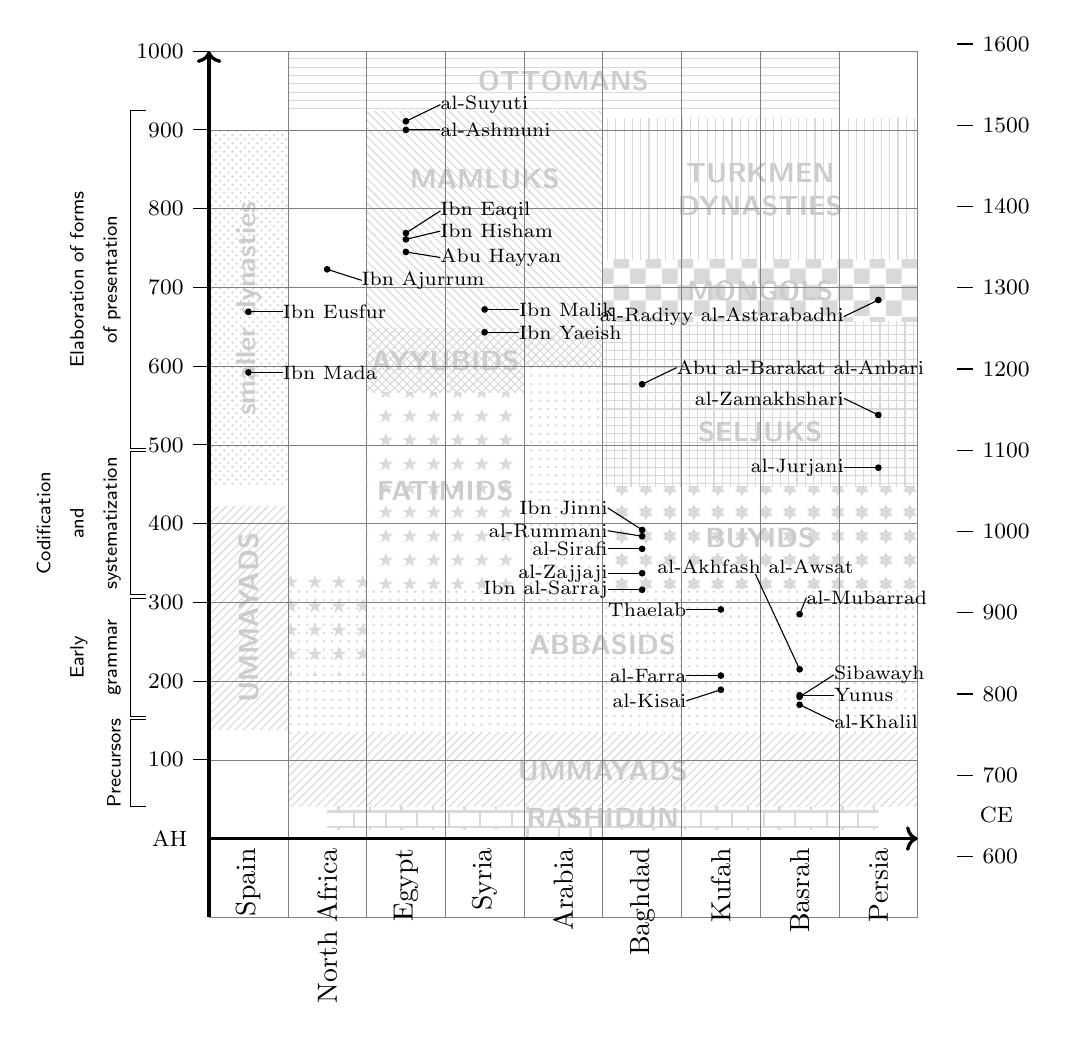
\begin{tikzpicture}[y=0.1mm]

\draw [help lines] (\beglong,\begah) grid (\endlong,\endah);

% Axis
\draw [->, very thick] (\beglong,0) -- (\endlong,0);
\draw [->, very thick] (0,\begah) -- (0,\endah);

% Axis ticks
\foreach \y in {100,200,...,\endah} {
  \draw (0, \y) -- (-.2, \y) node [anchor=east] {\footnotesize \y};
}
\node  at (-0.5,0) {\footnotesize AH};
\node  at (10,30) {\footnotesize CE};

\foreach \y in {600,700,...,1600} {
  \ceaxis{\y}
}


\foreach [count=\i] \x in \regions {
    %\node[label={\x}] (\i) at (\i-0.5, 0) {};
    \node[rotate=90,align=left,anchor=east] () at (\i-0.5, 0) {\x};
}
    %\node[align=left,anchor=east] () at (7.5, 180) {Sibawayhi\x};
    %\node[above right=10pt of {(7.5,180)}, outer sep=2pt,fill=white] {Spin distance=3mm,ibawayh};
    %\node [fill, draw, circle, minimum width=3pt, inner sep=0pt, pin={[fill=white, outer sep=2pt]135:{\scriptsize Fulan}}] at (3.5,300) {};
    %\node [fill, draw, circle, minimum width=2pt, inner sep=0pt, pin={[fill=white, outer sep=0pt]-45:{\scriptsize al-Khalil}}] at (7.5,170) {};
    %\node (khalil) [fill, draw, circle, minimum width=2pt, inner sep=0, outer sep=0] at (7.5,170) {};
    %\coordinate (khalil)  at (7.5,170) {};
    %\node [fill, draw, circle, minimum width=2pt, inner sep=0] at (7.5,170) {};
    %\node (khaliltext)  [inner sep=0, outer sep=0, right of=khalil, xshift=-1pt, yshift=-6pt] {\scriptsize al-Khalil};
    %\draw (khalil)  -- (khaliltext);
    % Baghdad
    \person{7.5}{170}{right}{west}{-16}{-6}{al-Khalil}
    \person{7.5}{180}{right}{west}{-16}{ 8}{Sibawayh}
    \person{7.5}{182}{right}{west}{-16}{ 0}{Yunus}
    \person{7.5}{215}{above}{south}{-16}{ 6}{al-Akhfash al-Awsat}
    \person{7.5}{285}{right}{west}{-26}{ 6}{al-Mubarrad}

    % Kufah
    %\person{6.5}{150}{left} {east}{ 16}{0}{Abu Hanifah}
    \person{6.5}{189}{left} {east}{ 16}{-4}{al-Kisai}
    \person{6.5}{207}{left} {east}{ 16}{0}{al-Farra}
    \person{6.5}{291}{left} {east}{ 16}{0}{Thaelab}

    % Baghdad
    \person{5.5}{316}{left} {east}{ 16}{0}{Ibn al-Sarraj}
    \person{5.5}{337}{left} {east}{ 16}{0}{al-Zajjaji}
    \person{5.5}{368}{left} {east}{ 16}{0}{al-Sirafi}
    \person{5.5}{384}{left} {east}{ 16}{2}{al-Rummani}
    \person{5.5}{392}{left} {east}{ 16}{8}{Ibn Jinni}
    \person{5.5}{577}{right} {west}{-16}{6}{Abu al-Barakat al-Anbari}

    % Syria
    \person{3.5}{643}{right} {west}{-16}{0}{Ibn Yaeish}
    \person{3.5}{672}{right} {west}{-16}{0}{Ibn Malik}

    % Egypt
    %\person{2.5}{204}{right} {west}{-16}{0}{al-Shafiei}
    \person{2.5}{745}{right} {west}{-16}{-2}{Abu Hayyan}
    \person{2.5}{761}{right} {west}{-16}{3}{Ibn Hisham}
    \person{2.5}{769}{right} {west}{-16}{8}{Ibn Eaqil}
    \person{2.5}{900}{right} {west}{-16}{0}{al-Ashmuni}
    \person{2.5}{911}{right} {west}{-16}{6}{al-Suyuti}

    % Persia
    \person{8.5}{471}{left} {east}{ 16}{0}{al-Jurjani}
    \person{8.5}{538}{left} {east}{ 16}{6}{al-Zamakhshari}
    \person{8.5}{684}{left} {east}{ 16}{-6}{al-Radiyy al-Astarabadhi}

    % Andalus
    \person{0.5}{592}{right}{west}{-16}{ 0}{Ibn Mada}
    \person{0.5}{669}{right}{west}{-16}{ 0}{Ibn Eusfur}

    % North Africa
    \person{1.5}{723}{right}{west}{-16}{-4}{Ibn Ajurrum}


    %\node [fill, draw, circle, minimum width=2pt, inner sep=0pt, pin={[pin distance=0.01mm,fill=white, outer sep=0pt]0:{\scriptsize Sibawayh d.\ 180}}] at (7.5,180) {};




    \dynasty    {bricks}           {5}    {5}      {0}     {11}  {}{} % Prophet pbuh
    \dynasty    {bricks}           {2.5}  {8.5}    {11}    {41}  {RASHIDUN}{}
    \dynasty    {north east lines} {2}    {9}      {41}    {132} {UMMAYADS}{}
    \dynasty    {north east lines} {1}    {1}      {\cetoah{756}}    {\cetoah{1031}} {UMMAYADS}{rotate=90}
    \dynasty    {dots}             {2}    {9}      {132}             {\cetoah{930}} {ABBASIDS}{yshift=6pt}
    \dynasty    {dots}             {5}    {5}      {\cetoah{909}}    {600} {}{}% Abbasids
    \dynasty    {fivepointed stars}{3}    {4}      {\cetoah{930}}    {\cetoah{1171}} {FATIMIDS}{}
    \dynasty    {fivepointed stars}{2}    {2}      {207}             {\cetoah{945}} {}{}
    \dynasty    {crosshatch}       {3}    {4}      {\cetoah{1171}}   {\cetoah{1250}} {AYYUBIDS}{}
    \dynasty    {crosshatch}       {5}    {5}      {600}             {\cetoah{1250}} {}{}
    \dynasty    {grid}             {6}    {9}      {\cetoah{1055}}   {\cetoah{1258}} {SELJUKS}{yshift=-10pt}
    \dynasty    {sixpointed stars} {6}    {9}      {\cetoah{930}}    {\cetoah{1055}} {BUYIDS}{}
    \dynasty    {checkerboard}     {6}    {9}      {\cetoah{1258}}   {\cetoah{1335}} {MONGOLS}{}
    \dynasty    {north west lines} {3}    {5}      {\cetoah{1250}}   {\cetoah{1517}} {MAMLUKS}{yshift=15pt}
    \dynasty    {crosshatch dots}  {1}    {1}      {\cetoah{1056}}   {\cetoah{1492}} {smaller dynasties}{rotate=90}
    \dynasty    {vertical lines}   {6}    {9}      {\cetoah{1335}}   {\cetoah{1508}} {TURKMEN\\ DYNASTIES}{}
    \dynasty    {horizontal lines} {2}    {8}      {\cetoah{1517}}   {1000} {OTTOMANS}{}

% Phases
% Data collection, formation, theroeticlaelaboration, consolidiation, degeneration
% \phase{Pre-theoretical\\grammar}{650}{780}
    \phase{\scriptsize Precursors}                           {\cetoah{660}} {\cetoah{770}}
    \phase{\scriptsize Early\\\scriptsize grammar}                        {\cetoah{770}} {\cetoah{920}}
    \phase{\scriptsize Codification\\\scriptsize and\\\scriptsize systematization}    {\cetoah{920}} {\cetoah{1100}}
    \phase{\scriptsize Elaboration of forms\\\scriptsize of presentation}{\cetoah{1100}}{\cetoah{1520}}



\end{tikzpicture}
\end{document}
